%\chapter{Preliminares. } % (fold)

El contenido de este capítulo abordará temas estrechamente relacionados con la criptografía, la seguridad de la información y las implicaciones que ésta podria traer si esta se encuentra corrompida por algun adversario. También, este capítulo contiene información acerca de los 2 tipos de criptografía que existen mencionando los diferentes esquemas de cifrado y los modos de operación que son utilizados por algunos de estos. De igual forma se describe con detalle los servicios que ofrece el cómputo nube, haciendo énfasis en un servicio en particular que es el de almacenamiento que se utilizará para la implementación de este protocolo criptogrráfico. 

\section{Definiciones. }
 \begin{itemize}

	\item \textbf{Criptografía. }
	 	La Criptografía es la ciencia que se encarga del estudio de técnicas matemáticas relacionadas con aspectos de seguridad  para transformar la información a una forma que no pueda entenderse a simple vista; sin embargo, el objetivo de la Criptografía no es sólo 	mantener los datos secretos, sino también protegerlos contra modificación y comprobar la fuente de los mismos ~\cite{menezes}.
	\item \textbf{Criptoanálisis. }
		Es la ciencia que se ocupa del análisis de un texto cifrado para obtener la información original sin conocimiento de la clave secreta, esto es, de forma ilícita rompiendo así los procedimientos de cifrado establecidos por la Criptografía, por lo que se dice que 		Criptoanálisis y Criptografía son ciencias complementarias pero contrarias. El criptoanálisis es el arte de descifrar comunicaciones cifradas sin conocer las llaves  ~\cite{cripto}.
 \end{itemize}

%==================================================================================================================================================================
\subsection{Servicios criptográficos. }
Los servicios criptográficos son aquellos que garantizan en un sistema de información la adquisición, almacenamiento, procesamiento y transmisión de la información y para lograrlo se valen de uno o más objetivos fundamentales. 
 \begin{itemize}
	\item \textbf{Confidencialidad. }
Es un servicio utilizado para mantener el contenido de la información de todos, excepto los autorizados a tenerla. El secreto es un término sinónimo de confidencialidad y privacidad.
Hay numerosos enfoques para proporcionar confidencialidad, que van desde la protección física a los algoritmos matemáticos que hacen que los datos sean ininteligibles.

	\item \textbf{Autenticación. }
Es un servicio relacionado con la identificación. Esta función se aplica tanto a las entidades como a la propia información. Dos partes que participan en una comunicación deben identificarse entre sí. La información entregada a través de un canal debe ser autenticada en cuanto al origen, fecha de origen, contenido de los datos, tiempo enviado, etc. Por estas razones este aspecto de la criptografía suele subdividirse en dos clases principales: autenticación de entidad y autenticación de origen de datos. La autenticación de origen de datos proporciona implícitamente la integridad de los datos (si se modifica un mensaje, la fuente ha cambiado).

	\item \textbf{Integridad. }
Es un servicio que se ocupa de la alteración no autorizada de los datos. Para asegurar la integridad de los datos, se debe tener la capacidad de detectar la manipulación de datos por parte de algún adversario. La manipulación de datos incluye cosas tales como inserción, supresión y sustitución.  

	\item \textbf{No repudio. }
Es un servicio que impide a una entidad negar compromisos o acciones anteriores. Cuando surgen disputas debido a que una entidad niega que se tomaron ciertas acciones, es necesario un medio para resolver la situación. Por ejemplo, una entidad puede autorizar la compra de una propiedad por otra entidad y posteriormente denegar que se concedió dicha autorización. Se necesita un procedimiento que involucre a un tercero de confianza para resolver la disputa  ~\cite{menezes}.
 \end{itemize}

%==================================================================================================================================================================
\section{Ataques a servicios criptográficos. }
Un ataque es una violación a la seguridad de la información realizada por intrusos que tienen acceso físico al sistema sin ningún tipo de restricción, su objetivo es robar la información o hacer que ésta pierda valor relativo, o que disminuyan las posibilidades de su supervivencia a largo plazo.

%Un intruso puede obtener información como:
%\begin{itemize}
%	\item Bloques de direcciones IP
%	\item Localización de sistemas críticos (DNSs, WINS, DHCPs, Servidores de correo, etc.)
%	\item Puntos de acceso para números telefónicos y VPNs
%	\item Información personal de los trabajadores de la organización
%	\item Organizaciones asociadas, subsidiarias, etc.
%\end{itemize}
%Existen dos tipos de ataques que amenazan las comunicaciones secretas:
%\begin{itemize}
%	\item Pasivo: es aquel en el cual el intruso sólo busca obtener la información y al hacerlo no la modifica, por lo que es difícil percatarse de que se está siendo atacado.
%	\item Activo: el intruso además de obtener la información la modifica de tal modo que sirva a sus intereses y al ser modificada es más fácil percatarse de que se está siendo atacado.
%Los ataques activos se dividen en dos tipos: Ataques a los métodos de cifrado y Ataques a los protocolos criptográficos.
%\end{itemize}

%\textbf{Ataques a los Métodos de Cifrado}
%Este tipo de ataques se realizan con la intención de obtener la clave secreta para poder descifrar libremente cualquier criptograma, para ello se aprovechan las vulnerabilidades que pudiera tener el método de cifrado.

 \begin{itemize} 
	\item \textbf{Ataque sólo con texto cifrado. }
Este caso es cuando el criptoanalista sólo conoce el criptograma y el algoritmo con que fue generado; con esta información pretende obtener el texto en claro.

	\item \textbf{Ataque con texto original conocido. }
En esta situación el criptoanalista conoce mensajes en claro seleccionados por él mismo y sus correspondientes criptogramas, así como el algoritmo con que éstos fueron generados; aquí el objetivo es conocer la clave secreta y poder descriptar libremente cualquier texto.

	\item \textbf{Ataque con texto cifrado escogido. }
El criptoanalista conoce el algoritmo de cifrado, así como un criptograma seleccionado por él mismo y su correspondiente texto en claro, su objetivo es obtener el mensaje en claro de todo criptograma que intercepte.

	\item \textbf{Ataque con texto escogido. }
En este caso el criptoanalista además de conocer el algoritmo de cifrado y el criptograma que quiere descriptar, también conoce el criptograma de un texto en claro que él elija y el mensaje en claro de un criptograma también elegido por él ~\cite{ataques}.
 \end{itemize}

%\subsection{Ataques a los Protocolos Criptográficos}
%Este tipo de ataques no pretenden encontrar la clave secreta para poder conocer el mensaje en claro, sino que buscan obtener la información vulnerando los protocolos criptográficos, es decir, pretenden burlar la serie de pasos establecidos para alcanzar los objetivos de seguridad y que tienen que ser realizados por las entidades involucradas en cierta comunicación. Ejemplos de este tipo de ataques son los siguientes:

%\textbf{Ataque con clave conocida}
%El atacante conoce claves utilizadas en cifrados anteriores y con base en ellas intenta determinar nuevas claves.

%\subsection{SUPLANTACIÓN DE PERSONALIDAD}
%El atacante asume la identidad de uno de los agentes autorizados en la red, y de esta manera obtiene libremente y sin tropiezos todos los mensajes en claro.

%\subsection{COMPILACIÓN DE UN DICCIONARIO}
%Un diccionario es un archivo guardado en la memoria de la computadora que contiene contraseñas cifradas de los usuarios autorizados en el sistema. Si el método de cifrado con que se cifran las claves es público, el atacante puede generar claves aleatorias y después cifrarlas con el objeto de encontrar alguna contenida en el diccionario (previamente obtenido). Cuando una clave generada por el atacante coincide con una contenida en el diccionario, se ha encontrado una clave de acceso al sistema, mediante el usuario correspondiente a la clave encontrada.

%\subsection{BÚSQUEDA EXHAUSTIVA}
%Este ataque se lleva a cabo generando aleatoriamente todos los valores posibles de las claves de acceso y probándolas hasta que una de ellas sea una clave válida en el sistema.

%\textbf{Ataque de hombre en medio}
%El intruso se filtra en la línea de comunicación entre dos agentes autorizados en la red; obtiene la información de uno de ellos y se la envía al otro usuario una vez que la ha utilizado.

%\subsection{Ataques en criptoanálisis}
%Aunque para validar la robustez de un criptosistema normalmente se suponen todas las condiciones del peor caso, existen ataques más específicos, en los que no se cumplen todas estas condiciones. Cuando el método de ataque consiste simplemente en probar todas y cada una de las posibles claves del espacio de claves hasta encontrar la correcta, nos encontramos ante un ataque de fuerza bruta o ataque exhaustivo. Si el atacante conoce el algoritmo de cifrado y sólo tiene acceso al criptograma, se plantea un ataque sólo al criptograma; un caso más favorable para el criptoanalista se produce cuando el ataque cumple todas las condiciones del peor caso; en este caso, el criptoanálisis se denomina de texto en claro conocido. Si además el atacante puede cifrar una cantidad indeterminada de texto en claro al ataque se le denomina de texto en claro escogido; este es el caso habitual de los ataques contra el sistema de verificación de usuarios utilizado por Unix, donde un intruso consigue la tabla de contraseñas (generalmente /etc/passwd) y se limita a realizar cifrados de textos en claro de su elección y a comparar los resultados con las claves cifradas (a este ataque también se le llama de diccionario, debido a que el atacante suele utilizar un fichero `diccionario' con los textos en claro que va a utilizar). El caso más favorable para un analista se produce cuando puede obtener el texto en claro correspondiente a criptogramas de su elección; en este caso el ataque se denomina de texto cifrado escogido. 

%Cualquier algoritmo de cifrado, para ser considerado seguro, ha de soportar todos estos ataques y otros no citados; sin embargo, en la criptografía, como en cualquier aspecto de la seguridad, informática o no, no debemos olvidar un factor muy importante: las personas. El sistema más robusto caerá fácilmente si se tortura al emisor o al receptor hasta que desvelen el contenido del mensaje, o si se le ofrece a uno de ellos una gran cantidad de dinero; este tipo de ataques (sobornos, amenazas, extorsión, tortura...) se consideran siempre los más efectivos. 


%==================================================================================================================================================================
\section{Criptografía Simétrica. }
Los esquemas criptográficos simétricos también se conocen como esquemas o algoritmos de clave simétrica, clave secreta y de clave única. Consideremos un esquema de cifrado que consiste en los conjuntos de transformaciones de cifrado y descifrado \textit{Ee: $e \in {\cal K}$} y \textit{Dd: $d \in {\cal K}$}, respectivamente, donde \textit{K} es el espacio clave. El esquema de cifrado se dice que es de clave simétrica si para cada par asociado de cifrado/descifrado de claves \textit{(e, d)}, es computacionalmente “fácil” para determinar \textit{d} conociendo sólo \textit{e}, y determinar \textit{e} a partir de \textit{d}. Desde\textit{ e = d} en los esquemas de cifrado de clave simétrica más prácticos, la clave simétrica término se convierte apropiado ~\cite{menezes}.
\\
Cuando exisen dos usuarios, que quieren comunicarse para compartir información a través de un canal inseguro que puede ser Internet, teléfonos móviles o comunicación LAN inalámbrica, etc, se presenta un problema, ya que existe algún adversario que tiene acceso a ese canal de comunicación, este tipo de escucha no autorizada se llama espionaje. En esta situación, la criptografía simétrica ofrece una solución: el usuario cifra su mensaje \textit{x} usando un algoritmo simétrico, dando el texto cifrado \textit{y}. El usuario destinatario recibe el texto cifrado y descifra el mensaje, si se tiene un algoritmo de cifrado fuerte, el texto cifrado se verá como bits aleatorios al adversario y no contendrá ninguna información que le sea útil ~\cite{paar}.


% La criptografía simétrica utiliza la misma clave para cifrar y descifrar el mensaje de datos, es decir se basa en un secreto compartido  ~\cite{sime}. \\ Características de la Criptografía simétrica: \begin{itemize}
%	\item La clave es la misma para cifrar que para descifrar un mensaje, por lo que sólo el emisor y el receptor deben conocerla.
%	\item Se basa en operaciones matemáticas sencillas, por ello son fácilmente implementados en hardware.
%	\item Debido al uso de operaciones basicas como son XOR y permutaciones son capaces de cifrar grandes cantidades de datos en poco tiempo en comparación con el uso de aritmética modular.
%			       \end{itemize} ~\cite{sime} 

Los algoritmos criptográficos simétricos tienen dos versiones: cifrador en bloque y cifrador de flujo. El beneficio del uso de un algoritmo simétrico radica en el procesamiento rápido para cifrar y descifrar un alto volúmen de datos. El cifrado simétrico es una táctica eficaz de almacenamiento de información sensible en una base de datos, un registro o archivo  ~\cite{sime}. 
\\  \\
Así como la criptografía tiene grandes ventajas para la solución en la comunicación de dos agentes a través de un canal inseguro, también cuenta con ciertas desventajas que son: 

\begin{itemize}
	\item La seguridad depende de un secreto compartido entre el emisor y el receptor.
	\item La administración de las claves no es escalable.
	\item La distribución manual de llaves es costosa, ocupa mucho tiempo y es propensa a errores.
	\item La distribución de claves debe hacerse a través de algún medio seguro como centros de distribución de llaves, implementación de algoritmos, etc ~\cite{ventajasime}. 
\end{itemize}

El esquema de cifrado simétrico se puede representar a través de la siguiente figura ~\ref{fig:2-3-1}.
\begin{figure}[H]
\centering
	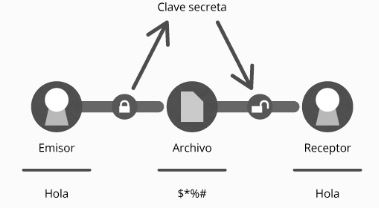
\includegraphics[width=10cm, height=5cm]{./images/Cripto_Simetrica.jpg}
	\caption{Diagrama de Criptografía Simétrica.}
	\label{fig:2-3-1}
\end{figure}


%La sintaxis de un esquema de cifrado simétrico, esta dada por la siguiente definición.
%\begin{definition} 
%Un esquema de cifrado simétrico está conformado por una tripleta de algoritmos 
%$\sf \Pi=(Gen, Enc, Dec)$, definidos como se describe a continuación:
%\begin{itemize}
%\item  El algoritmo generador de claves $\sf Gen$ selecciona una llave  $K$ al azar del conjunto de llaves $\cal K$, esto se denotará como $K \rand {\cal K}$.
%Esta clave $K$  será usada por los algoritmos  $\sf Enc$ y $\sf Dec$, esta clave la compartirán  emisor y receptor. 
%\item El algoritmo de cifrado $\sf Enc$, toma como entrada un texto en claro  $M \in {\cal M}$ y una clave $K$ generada por  $\sf Gen$  y regresa un texto cifrado $C \in {\cal C}$.  Usualmente esto se denota como $C \leftarrow {\sf Enc}_K(M)$.
 %\item El algoritmo de descifrado $\sf Dec$, toma como entrada un texto cifrado $C$ y una llave $K$ y regresa $M$. Esta operación se denota por  $M \leftarrow {\sf Dec}_K(C)$.
%Para que cualquier algoritmo de cifrado simétrico funcione correctamente, se debe garantizar que para
%todas las llaves posibles en  $\cal K$ y todos los posibles mensajes $\cal M$, $$ {\sf Dec}_K({\sf Enc}_K(M)) = M.$$
%\end{itemize}
%\end{definition}

%==================================================================================================================================================================
\section{Criptografía Asimétrica. }
En el modelo clásico de criptografía, dos entidades escogen secretamente la clave \textit{K}. \textit{K} da lugar a una regla de cifrado \textit{ek} y una regla de descifrado \textit{dk}. En este criptosistema, \textit{dk} es el mismo que \textit{ek} o fácilmente derivado de él, a este se le llama criptosistema de clave simétrica, ya que la exposición de cualquiera \textit{ek} o \textit{dk} hace que el sistema sea inseguro. Un inconveniente de un sistema de clave simétrica es que requiere la comunicación previa de la clave \textit{K} entre estas dos entidades, utilizando un canal seguro antes de que se transmita cualquier texto cifrado ~\cite{stinson}.
\\
La idea detrás de un criptosistema de clave pública es que podría ser posible encontrar un criptosistema donde es computacionalmente imposible determinar \textit{dk} dado \textit{ek}.Si es así, entonces la regla de cifrado \textit{ek} es una clave pública que podría ser publicada en un directorio, por ejemplo (de ahí el término sistema de clave pública). La ventaja de un sistema de clave pública es que una entidad puede enviar un mensaje cifrado a otra entidad (sin la comunicación previa de una clave secreta compartida) utilizando la regla de cifrado pública \textit{ek}. La entidad que recibe la comunicación será la única que puede descifrar el texto cifrado, utilizando la regla de descifrado \textit{dk}, que se llama la clave privada ~\cite{stinson}.
\\ 
Sea  \textit{Ee: $e \in {\cal K}$} un conjunto de transformaciones de cifrado, y sea \textit{Dd: $d \in {\cal K}$} el conjunto de transformaciones de descifrado correspondientes, donde  \textit{K} es el espacio clave. Considere cualquier par de transformaciones asociadas de cifrado/descifrado  \textit{(Ee, Dd)} y suponga que cada par tiene la propiedad de que saber  \textit{Ee} es computacionalmente inviable, dado un texto cifrado$c \in {\cal C}$, para encontrar el mensaje $m \in {\cal M}$ tal que \textit{Ee (m) = C}. Esta propiedad implica que dada \textit{e} es imposible determinar la clave de descifrado correspondiente \textit{d}. (Por supuesto, \textit{e} y \textit{d} son simplemente medios para describir las funciones de cifrado y descifrado, respectivamente) ~\cite{menezes}.

El cifrado asimétrico puede ser representado como aparece en la figura ~\ref{fig:2-4-1}.

\begin{figure}[H]
\centering
	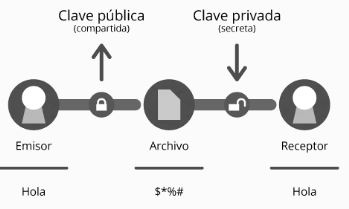
\includegraphics[width=10cm, height=5cm]{./images/Cripto_Asimetrica.jpg}
	\caption{Diagrama de Criptografía Asimétrica.}
	\label{fig:2-4-1}
\end{figure}

 Los beneficios de la criptografía asimétrica son la solución a los problemas de la criptografía simétrica, pues las claves públicas pueden ser distribuidas con toda tranquilidad, no valen de nada sin las claves privadas. El cifrado asimétrico se emplea muy frecuentemente para pasar con seguridad una clave privada, que posteriormente, será la que se utilice para cifrar y/o descifrar otra información.

%==================================================================================================================================================================
\section{Cifrado por bloques. }
Los algoritmos de cifrado por bloques toman bloques de tamaño fijo del texto en claro y producen un bloque de tamaño fijo de texto cifrado, generalmente del mismo tamaño que la entrada. El tamaño del bloque debe ser lo suficientemente grande como para evitar ataques de texto cifrado. La asignación de bloques de entrada a bloques de salida debe ser uno a uno para hacer el proceso reversible y parecer aleatoria.\\ 
Para la asignación de bloques los algoritmos de cifrado simétrico realizan sustituciones y permutaciones en el texto en claro hasta obtener el texto cifrado.\\ 
La sustitución es el reemplazo de un valor de entrada por otro de los posibles valores de salida, en general, si usamos un tamaño de bloque k, el bloque de entrada puede ser sustituido por cualquiera de los bloques posibles.
La permutación es un tipo especial de sustitución en el que los bits de un bloque de entrada son reordenados para producir el bloque cifrado, de este modo se preservan las estadísticas del bloque de entrada (el número de unos y ceros). \\ \\  Los algoritmos de cifrado por bloques iterativos funcionan aplicando en sucesivas rondas una transformación a un bloque de texto en claro. La misma función es aplicada a los datos usando una subclave obtenida de la clave secreta proporcionada por el usuario. El número de rondas en un algoritmo de cifrado por bloques iterativo depende del nivel de seguridad deseado.

La sustitución es el reemplazo de un bloque de $n$ bits por otro bloque de $n$ bits en un espacio de 
$2^{k}$~\cite{bloc}. Los cifradores por bloques mas usados son AES (Advanced Encryption Standard, por sus 
siglas en ingl\'es) y DES (Data Encryption Standard, por sus siglas en ingl\'es). ~\cite{bloques}\\ \\ 

Los cifradores por bloques pueden ser representados como se ve en la figura ~\ref{fig:2-5-1}.

\begin{figure}[H]
\centering
	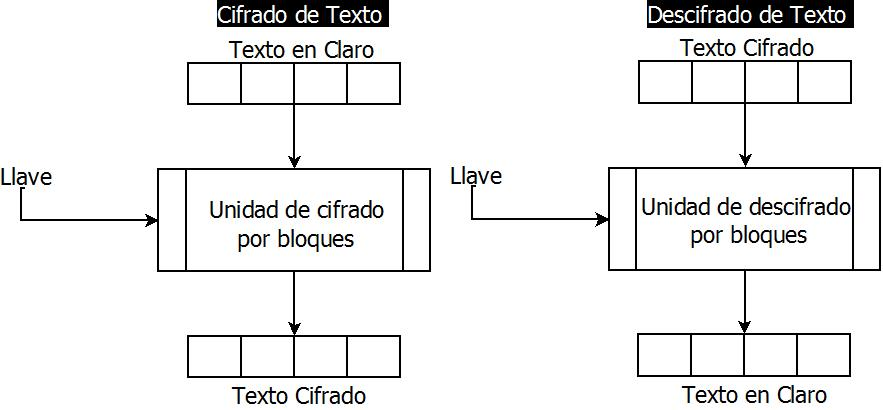
\includegraphics[width=10cm, height=5cm]{./images/CifradoBloques.jpeg}
	\caption{Diagrama de Cifradores por Bloques}
	\label{fig:2-5-1}
\end{figure}



%\section{Modos de operación. }
%Un modo de operación es una técnica para mejorar el efecto de un algoritmo criptográfico o adaptar el algoritmo para una aplicación, tal como aplicar un cifrador por bloques a una secuencia de bloques de datos o un flujo de datos. Los cuatro modos están destinados a cubrir virtualmente todas las aplicaciones posibles de cifrado para las cuales se podría usar un cifrador por bloques. A medida que han aparecido nuevas aplicaciones y requisitos, el NIST  (National Institute of Standards and Technology) ha ampliado la lista de modos recomendados a cinco en la Publicación Especial 800-38A. Estos modos están diseñados para usarse con cualquier cifrador por bloques bloques, incluyendo DES triple y AES.\\\\


%\textit{CBC}(Cipher-block chaining): La entrada al algoritmo de cifrado es el XOR de los siguientes 64 bits de texto plano y los 64 bits de cifrado anteriores.\\
%\begin{itemize}
%	\item La salida de uno de los bloques de cifrado se mete a otro bloque de cifrado junto con el siguiente bloque de mensaje.
%	\item Toma como entradas un vector de inicialización (IV) y un bloque de mensaje (m).
%	\item Durante el cifrado la salida del i - ésimo bloque depende del anterior i -1 bloques.
%	\item La salida de cada uno de los bloques depende de todo lo anterior y esto lo hace mas seguro que ECB.
%	\item  El descifrado de CBC es no secuencial.
%\end{itemize}

%\begin{figure}[h]
    %\centering
%    \begin{subfigure}[t]{0.5\textwidth}
    %    \centering
        %\includegraphics[height=3in]{./images/CBC.png}
%        \caption{Diagrama CBC Cifrado / Descfrado.}
    %    \label{fig:1-3-1}
%    \end{subfigure}
%\end{figure}
%\pagebreak

%\textit{CFB}(Cipher Feedback): La entrada se procesa j bits a la vez. El texto cifrado precedente se utiliza como entrada al algoritmo de cifrado para producir la salida pseudoaleatoria, que se le aplica XOR con el texto sin formato para producir la siguiente unidad de texto cifrado.\\
%\begin{itemize}
%	\item Los bloques de cifrado también están encadenados pero la salida es muy diferente a los demás.
%	\item Para cada bloque, el cifrado es producido haciendo XOR con el mensaje.
%	\item Una ventaja de implementación es que no es necesaria la operación de descifrar no es necesario.
%\end{itemize}

%\begin{figure}[h]
    %\centering
%    \begin{subfigure}[t]{0.5\textwidth}
    %    \centering
        %\includegraphics[height=3in]{./images/CFB.png}
     %   \caption{Diagrama CFB Cifrado}
        %\label{fig:1-3-1}
%    \end{subfigure}
%\end{figure}
%\pagebreak

%\textit{OFB}(Output feedback): Similar a CFB, excepto que la entrada al algoritmo de cifrado es la salida DES anterior.\\
%\begin{itemize}
%	\item En OFB la salida del bloque de cifrado es alimentada de nuevo en la siguiente bloque de cifrado.
%	\item El IV es cifrado varias veces para obtener una corriente de bytes aleatorios.
%	\item Estas corrientes de bytes aleatorios se les hace XOR con el texto en plano para generar el texto cifrado.
%\end{itemize}

%\begin{figure}[h]
%    \centering
    %\begin{subfigure}[t]{0.5\textwidth}
%        \centering
 %       \includegraphics[height=3in]{./images/OFB.png}
     %   \caption{Diagrama OFB Cifrado}
        %\label{fig:1-3-1}
%    \end{subfigure}
%\end{figure}
%\pagebreak

%\textit{CTR}(Counter): Cada bloque de texto sin formato se le aplica XOR con un contador cifrado. El contador se incrementa para cada bloque subsiguiente.\\
%\begin{itemize}
%	\item CTR toma un vector de inicialización (IV) y en cada iteración el valor de IV se incrementa en 1 y queda cifrado.
%	\item Para obtener el mensaje cifrado se hace una XOR con el IV y el bloque de mensaje.
%	\item En términos de eficiencia CTR es mejor que CBC, OFB o CFB, ya que en este modo se pueden hacer las operaciones en paralelo ya que no dependen de algo para poder ser cifradas.
%\end{itemize}

%\begin{figure}[h]
    %\centering
%    \begin{subfigure}[t]{0.5\textwidth}
    %    \centering
        %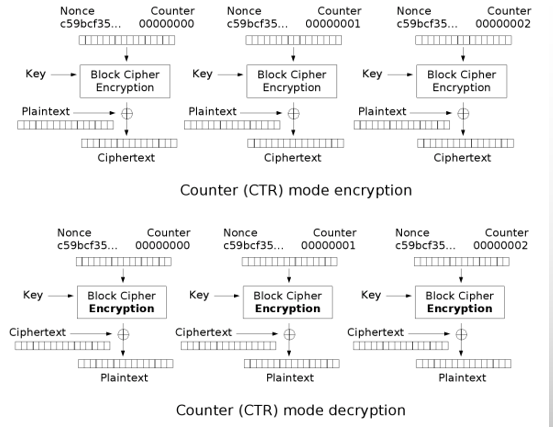
\includegraphics[height=3in]{./images/CTR.png}
%        \caption{Diagrama CTR Cifrado}
%        \label{fig:1-3-1}
    %\end{subfigure}
%\end{figure}

%\pagebreak

%==================================================================================================================================================================

\section{Ataques de fuerza bruta}

Los ataques de fuerza bruta se basan en un concepto simple: Oscar, el atacante, obtiene el texto cifrado escuchando en el canal y pasa a tener un pedazo corto del texto claro, por ejemplo, el encabezado de un archivo que fue cifrado. Oscar ahora simplemente descifra el primer pedazo del texto cifrado con todas las claves posibles. Si el texto claro resultante coincide con el pedazo corto del texto claro, sabe que ha encontrado la clave correcta.\\

\begin{definition} 
Ataque de fuerza bruta\\
Sea \textit{(x, y)} el texto claro y el texto cifrado, y sea \textit{K = [K1, ..., Kk]} el espacio clave de todas las claves posibles \textit{ki}. Un ataque de fuerza bruta comprueba que para cada \textit{ki $\in$ K} si \\
\textit{ \[d_{ki}(y) = x\] }.\\
Si la igualdad se mantiene, se encuentra una posible clave correcta; Si no, se procede con la siguiente clave.\\
\end{definition}
En la práctica, un ataque de fuerza bruta puede ser más complicado porque las claves incorrectas pueden dar resultados positivos falsos. \\
Es importante señalar que un ataque de fuerza bruta contra cifrados simétricos es siempre posible en un principio. Si es factible en la práctica depende del espacio clave, es decir, en el número de posibles claves que existen para un cifrado dado. Si se están probando todas las claves en muchas computadoras modernas toma demasiado tiempo, es decir, varias décadas, el cifrado es computacionalmente seguro contra un ataque de fuerza bruta ~\cite{paar}.\\



%==================================================================================================================================================================


\section{RSA}

El esquema de criptografía RSA, a veces denominado algoritmo Rivest-Shamir-Adleman, es actualmente el esquema criptográfico asimétrico más utilizado, aunque las curvas elípticas y los esquemas de logaritmos discretos están ganando terreno. RSA fue patentado en los Estados Unidos (pero no en el resto del mundo) hasta el 2000. La función unidireccional subyacente de RSA es el problema de factorización de enteros: Multiplicar dos grandes primos es computacionalmente fácil (de hecho, se puede hacer con
Papel y lápiz), pero factorizar el producto resultante es muy difícil, el teorema de Euler y la función $\varphi$ de Euler desempeñan papeles importantes en RSA ~\cite{paar}.
\\
Hay muchas aplicaciones para RSA, pero en la práctica se usa con más frecuencia para:

	\begin{itemize}
		\item Cifrado de pequeñas piezas de datos, especialmente para el transporte de claves.
		\item Las firmas digitales, por ejemplo, para certificados digitales en Internet ~\cite{paar}.
	\end{itemize}

\textbf{Cifrado y descifrado} \\
El cifrado y descifrado RSA se realiza en el campo de los numeros enteros \textit{Zn} y los cálculos modulares desempeñan un papel central. RSA cifra el texto en claro \textit{x}, donde consideramos que la cadena de bits que representa \textit{x} es un elemento en \textit{Zn} = {0,1, ..., n-1}. Como consecuencia, el valor binario del texto en claro \textit{x} debe ser menor que \textit{n}. Lo mismo ocurre con el texto cifrado. El cifrado con la clave pública y el descifrado con la clave privada son los siguientes:
\\ \\
\textbf{\textit{Cifrado RSA}}\\ Dada la clave pública \textit{(n, e) = kpub} y el texto en claro \textit{x}, la función de cifrado es:
\\
\textit{ y = $ek_{pub}$ (x) $\equiv$ $x^{2}$ mod n }\\
Donde:  x,y $\in$ \textit{Zn}


\textbf{\textit{Descifrado RSA}} \\Dada la clave privada \textit{d = Kpr} y el texto cifrado \textit{y}, la función de descifrado es:
\\
\textit{ x = $dk_{pr}$ (y) $\equiv$ $y^{d}$ mod n }\\
Donde:  x,y $\in$ \textit{Zn} ~\cite{paar}. \\


 \textbf{Generación de llaves} \\
Estos son los pasos involucrados en el cálculo de la clave pública y privada para un criptosistema RSA.
\begin{itemize}

	\item Elegir 2 números primos grandes \textit{p} y \textit{q}.
	\item Calcular \textit{n = p $\cdot$ q }.
	\item Calcular \textit{$\varphi$ (n) = (p - 1)(q - 1)}.
	\item Seleccionar la clave pública \textit{e} $\in$ {1,2,...., $\varphi$ (n) - 1} tal que \\ \textbf{\textit{gcd(e,$\varphi$(N))=1}}.
	\item Calcular la clave privada \textit{d} tal que, \textit{d $\cdot$ e $\equiv$ mod $\varphi$ (n)} ~\cite{paar}. \\
\end{itemize} 


\textbf{Requisitos para el criptosistema RSA:}
\begin{itemize}
	\item Dado que un atacante tiene acceso a la clave pública, debe ser computacionalmente imposible determinar la clave privada  \textit{d} dados los valores de clave pública  \textit{e} y  \textit{n}.
	\item Como  \textit{x} es único hasta el tamaño del módulo  \textit{n}, no podemos cifrar más de  \textit{l} bits con un cifrado RSA, donde  \textit{l} es la longitud de bits de  \textit{n}.
	\item Debe ser relativamente fácil calcular  \textit{x $\cdot$ e mod n}, es decir, cifrar y  \textit{y $\cdot$ d mod n}, es decir, descifrar. Esto significa que necesitamos un método para una rápida exponenciación con números grandes.
	\item Para un \textit{n} dado, debe haber muchos pares de clave privada / clave pública, de lo contrario un atacante podría ser capaz de realizar un ataque de fuerza bruta. (Resulta que esta exigencia es fácil de satisfacer.) ~\cite{paar}.
\end{itemize}

%==================================================================================================================================================================
\section{Firmas a ciegas. }

Las firmas a ciegas son un tipo especial de firmas digitales en las que se firma algo que no se conoce. Para hacer firmas a ciegas se utilizan factores de opacidad, para ocultar el mensaje original que se requiere que esté firmado, y así la autoridad no pueda conocer lo que está firmando.
Por lo tanto, el propósito de una firma a ciegas es evitar que el firmante B conozca el mensaje que firma; y así posteriormente, sea incapaz de asociar el mensaje que firmó con el remitente A. Entonces, las firmas a ciegas tienen aplicación en varias situaciones. A continuación se mencionan dos de ellas:
\begin{itemize}
	\item Cuando se utiliza dinero electrónico. En este caso, m representa un valor monetario que A (el cliente) tiene derecho a gastar. Y así, cuando m y s(m) se presentan a B (el banco) para efectuar el pago, B es incapaz de identificar al cliente que originalmente le dio ese dinero electr´onico a firmar, pues le fue enviado de manera oculta. Lo anterior permite que la identidad de A permanezca anónima, y sus movimientos financieros no puedan ser monitoreados.
	\item En las elecciones electrónicas también pueden utilizarse las firmas a ciegas, ya que se requiere que B (una autoridad electoral) no conozca la identidad de A (el votante) debido a que el voto debe efectuarse de manera anónima. Sin embargo, es necesario que A demuestre que su voto m es válido. Lo cual se logra cuando A presenta ante B la firma s(m). Y se sabe de antemano que B no puede asociar s(m) a A, debido a que el votante previamente le envió a B su voto m pero de forma oculta para que se lo firmara. ~\cite{ciegas}
\end{itemize} 

%==================================================================================================================================================================
\section{Funciones Hash. }
A continuación se describirán las características de las {\it funciones hash}, también conocidas como {\it funciones de resumen}. Las funciones hash basan su definición en funciones de un solo sentido  ({\it one-way functions}, en inglés). Una función de un solo sentido es aquella que para un valor $x$, es  muy fácil calcular $f(x)$, pero es muy difícil hallar $f^{-1}(x)$. Es complicado en general, hallar funciones de este tipo y probar que lo son.
\begin{definition}
Una función hash, es una función de un solo sentido cuya entrada $m$  es un mensaje de longitud arbitraria y la salida es una cadena binaria de longitud fija. Al resumen o hash de un mensaje $m$, se le denotará como $h(m)$. Una función hash debe
tener las siguientes propiedades:
\begin{itemize}
	\item Para cualquier mensaje $m$, debe ser posible calcular $h(m)$ eficientemente. 
	\item Dado $h(m)$, debe ser computacionalmente difícil, hallar un mensaje $m'$, tal que $h(m)=h(m')$.
	\item Debe ser computacionalmente difícil, hallar dos mensajes $m$ y $m'$ tales que $h(m)=h(m')$.
\end{itemize}
\end{definition}
 
Entre las funciones hash que se usan para criptograf\'ia est\'an: MD2, MD4, MD5, donde MD significa {\it Message Digest}, y el algoritmo est\'andar al momento de escribir \'estas notas es el {\it Secure Hash Algorithm} por sus siglas en ingl\'es SHA.
  La MD5 fue dise\~nada por Ron Rivest, toma como entrada un mensaje de longitud arbitraria y proporciona como salida una cadena binaria de 128 bits.
El mensaje de entrada se procesa por bloques de 512 bits.  La SHA 256 fue dise\~nada por en NIST (National Institute of Standards and Technology) y se estableci\'o como est\'andar en 1993. Recibe como entrada un mensaje con longitud menor a $2^{64}$ bits y
como salida se obtiene una cadena binaria de 160 bits. Al igual que el MD5, se procesa en bloques de 512 bits ~\cite{modes}.


%==================================================================================================================================================================
\section{Cómputo Nube. }
El cómputo nube definido así por el NIST, es un modelo para permitir un acceso a la red ubicuo, es decir, que se encuentra presente en todas partes al mismo tiempo y conveniente a un conjunto de recursos informáticos configurables (por ejemplo, redes, servidores, almacenamiento, aplicaciones y servicios) que se puede aprovisionar y liberar rápidamente con un esfuerzo mínimo de gestión o una interacción entre el proveedor de servicios.
Este modelo de cómputo nube se compone de 5 características esenciales, 3 modelos de servicio y 4  modelos de despliegue. \\ \\  


\textbf{Características: }
\begin{itemize}
	\item \textbf {Auto-servicio bajo demanda. } \\  Un consumidor puede proporcionar unilateralmente capacidades del tiempo del servidor y el almacenamiento en red, según se necesite automáticamente sin interacción con cada proveedor de servicios.
 	\item \textbf {Amplio acceso a la red. } \\   Las capacidades están disponibles a través de la red y se accede a través de mecanismos que promueven el uso por plataformas de clienteheterogéneas finas o gruesas (por ejemplo, teléfonos móviles, tablets, computadoras portátiles y estaciones de trabajo)
	\item \textbf {Agrupación de recursos. } \\ Los recursos informáticos del proveedor se agrupan para servir a múltiples consumidores utilizando un modelo de múlti- usuario, con diferentes recursos físicos y virtuales asignados dinámicamente y reasignados de acuerdo con la demanda del consumidor. Hay una sensación de independencia de ubicación en que el cliente generalmente no tiene control o conocimiento sobre la ubicación exacta de los recursos proporcionados, pero puede especificar la ubicación en un nivel superior de abstracción (por ejemplo, país, estado o centro de datos). Ejemplos de recursos incluyen almacenamiento, procesamiento, memoria y ancho de banda de la red.
	\item \textbf{Elasticidad rápida. } \\ Las capacidades pueden ser suministradas elásticamente y liberadas, en algunos casos de forma automática, para escalar rápidamente hacia fuera y hacia adentro proporcional a la demanda. Para el consumidor, las capacidades disponibles para la provisión a menudo parecen ser ilimitadas y pueden ser apropiadas en cualquier cantidad en cualquier momento.
	\item \textbf{Servicio medido. } \\ Los sistemas de cómputo nube controlan y optimizan automáticamente el uso de recursos aprovechando una capacidad de medición en algún nivel de abstracción apropiado al tipo de servicio (por ejemplo, almacenamiento, procesamiento, ancho de banda y cuentas de usuario activas). El uso de recursos puede ser monitoreado, controlado y reportado, proporcionando transparencia tanto para el proveedor como para el consumidor del servicio utilizado.
\end{itemize}    


 \textbf{Modelos de servicio. }

\begin{itemize}
	\item \textbf {Software como Servicio (SaaS). } \\ La capacidad proporcionada al consumidor es utilizar las aplicaciones del proveedor que se ejecutan en una infraestructura en la nube. Las aplicaciones son accesibles desde varios dispositivos cliente a través de una interfaz de cliente ligero, como un navegador web (por ejemplo, correo electrónico basado en web) o una interfaz de programa. El consumidor no gestiona ni controla la infraestructura oculta de la nube, incluyendo la red, los servidores, los sistemas operativos, el almacenamiento o incluso las capacidades de las aplicaciones individuales, con la posible excepción de las limitadas configuraciones específicas de la configuración de la aplicación.
	\item \textbf {Plataforma como Servicio (PaaS). } \\ La capacidad proporcionada al consumidor es desplegar en la infraestructura de la nube aplicaciones creadas por el consumidor, utilizando lenguajes de programación, bibliotecas, servicios y herramientas soportadas por el proveedor. El consumidor no gestiona ni controla la infraestructura oculta de la nube, incluyendo la red, los servidores , sistemas operativos o de almacenamiento, pero tiene control sobre las aplicaciones desplegadas y, posiblemente, configuración de configuración para el entorno de alojamiento de aplicaciones.
	\item \textbf {Infraestructura como Servicio (IaaS). } \\  La capacidad proporcionada al consumidor es proveer procesamiento, almacenamiento, redes y otros recursos de computación fundamentales donde el consumidor es capaz de desplegar y ejecutar software arbitrario, que puede incluir sistemas operativos y aplicaciones. El consumidor no gestiona ni controla la infraestructura subyacente de la nube, sino que tiene control sobre los sistemas operativos, el almacenamiento y las aplicaciones implementadas; Y posiblemente un control limitado de componentes de red selectos (por ejemplo, firewalls de host). 
\end{itemize}  



 \textbf{Modelos de despliegue. }
\begin{itemize}
	\item \textbf {Nube privada. } \\ La infraestructura de la nube está preparada para el uso exclusivo de una sola organización que comprende varios consumidores (por ejemplo, unidades de negocio). Puede ser propiedad, administrado y operado por el órgano.
	\item \textbf{Nube de la comunidad. } \\ La infraestructura de la nube está preparada para uso exclusivo por una comunidad específica de consumidores de organizaciones que tienen preocupaciones compartidas (por ejemplo, misión, requisitos de seguridad, política y consideraciones de cumplimiento). Puede ser propiedad, administrado y operado por una o más de las organizaciones de la comunidad, un tercero, o una combinación de ellos, y puede existir dentro o fuera de las instalaciones.
	\item \textbf{Nube pública. } \\ La infraestructura de la nube está preparada para el uso abierto por el público en general. Puede ser propiedad, administrado y operado por una organización comercial, académica u gubernamental, o alguna combinación de ellos. Existe en las instalaciones del proveedor de la nube.
	\item \textbf{Nube híbrida. } \\  La infraestructura de la nube es una composición de dos o más infraestructuras de nube distintas (privadas, comunitarias o públicas) que siguen siendo entidades únicas, pero están unidas por una tecnología estandarizada o propietaria que permite la portabilidad de datos y aplicaciones (por ejemplo, burbujas de nube para equilibrar la carga entre Nubes).
\end{itemize}   




 \textbf{Problemas en Cómputo Nube. }

\begin{itemize}
	%\item \textbf {Abuso y mal uso del Cómputo Nube. } \\ Esta amenaza afecta principalmente a los modelos de servicio IaaS y PaaS y se relaciona con un registro de acceso a estas infraestructuras/plataformas poco restrictivo. Es decir, cualquiera con una tarjeta de crédito válida puede acceder al servicio, con la consecuente proliferación de spammers, creadores de código malicioso y otros criminales que utilizan la nube como centro de operaciones. 
	\item \textbf {Interfaces y API poco seguros. } \\ Generalmente los proveedores de servicios en la nube ofrecen una serie de interfaces y API (del inglés, Application Programming Interface) para controlar e interactuar con los recursos. De este modo, toda la organización, el control, la provisión y la monitorización de los servicios cloud se realiza a través de estos API o interfaces. 
Dado que todo (autenticación, acceso, cifrado de datos, etc.) se realiza a través de estas herramientas, se hace necesario que los interfaces estén diseñados de forma segura, evitando así los problemas de seguridad, tanto los que son intencionados como los que se producen de forma accidental. 
	%\item \textbf {Amenaza Interna. } \\ Como en todos los sistemas de información, la amenaza que suponen los propios usuarios es una de las más importantes, dado que tienen acceso de forma natural a los datos y aplicaciones de la empresa. En un entorno cloud esto no es en absoluto diferente ya que se pueden desencadenar igualmente incidentes de seguridad provocados por empleados descontentos y accidentes por error o desconocimiento. 
%Además, en muchos casos, es el propio proveedor del servicio el que gestiona las altas y bajas de los usuarios, produciéndose brechas de seguridad cuando el consumidor del servicio no informa al proveedor de las bajas de personal en la empresa. 
%Como es lógico, estos incidentes repercuten de forma importante en la imagen de la empresa y en los activos que son gestionados. 
%Los proveedores de servicio deberán proveer a los consumidores del servicio de medios y métodos para el control de las amenazas internas.
	%\item \textbf {Problemas derivados de la tecnología compartida. } \\  Esta amenaza afecta a los modelos IaaS, ya que en un modelo de Infraestructura como Servicio los componentes físicos (CPU, GPU, etc.) no fueron diseñados específicamente para una arquitectura de aplicaciones compartidas. Se han dado casos en los que los hipervisores de virtualización podían acceder a los recursos físicos del anfitrión provocando, de esta forma, incidentes de seguridad. 
%Para evitar este tipo de incidentes se recomienda implementar una defensa en profundidad con especial atención a los recursos de computación, almacenamiento y red. Además, se ha de generar una buena estrategia de seguridad que gestione correctamente los recursos para que las actividades de un usuario no puedan interferir en las del resto. 
	\item \textbf {Pérdida o fuga de información. } \\ Existen muchas formas en las que los datos se pueden ver comprometidos. Por ejemplo, el borrado o modificación de datos sin tener una copia de seguridad de los originales, supone una pérdida de datos. 
En la nube, aumenta el riesgo de que los datos se vean comprometidos ya que el número de interacciones entre ellos se multiplica debido a la propia arquitectura de la misma. Esto deriva en pérdida de imagen de la compañía, daños económicos y, si se trata de fugas, problemas legales, infracciones de normas, etc.
	\item \textbf {Secuestro de sesión o servicio. } \\  En un entorno en la nube, si un atacante obtiene las credenciales de un usuario del entorno puede acceder a actividades y transacciones, manipular datos, devolver información falsificada o redirigir a los clientes a sitios maliciosos.
	%\item \textbf {Riesgos por desconocimiento. } \\ Uno de los pilares de las infraestructuras cloud es reducir la cantidad de software y hardware que tienen que adquirir y mantener las compañías, para así poder centrarse en el negocio. Esto, si bien repercute en ahorros de costes tanto económicos como operacionales, no puede ser motivo para el deterioro de la seguridad por falta de conocimiento de esta infraestructura. 
%Para asistir en la toma de decisiones sobre las medidas de seguridad que se han de implantar en un entorno cloud es conveniente conocer, al menos en parte, la información técnica de la plataforma. Datos como con quién se comparte la infraestructura o los intentos de acceso no autorizados pueden resultar muy importantes a la hora de decidir la estrategia de seguridad. 
%La carencia de información de este tipo puede derivar en brechas de seguridad desconocidas por el afectado. 
\end{itemize} 


%Las funciones hash son usadas para construir una pequeña huella digital de la informaci\'on, si la informaci\'on es alterada tambi\'en la huella digital es alterada. Esta caracter\'istica hace que las funciones hash sean ampliamente usadas para verificar la integridad de datos.\\
%De manera formal, un funci\'on Hash es una Cuadrupla$(X,Y,K,H)$ donde:
%\begin{enumerate}
% \item $X$ es un conjunto de posibles mensajes.
% \item $Y$ es un conjunto finito de posibles resúmenes de mensajes o etiquetas de autenticación.
% \item $K$, el espacio de claves, es un conjunto finito de posibles claves.
% \item Para cada $k\quad \epsilon\quad K$, existe una función hash $h_k\quad \epsilon\quad H$. Parac ada $h_k: X \longrightarrow Y$.
% \cite{stinson}
%\end{enumerate}



